
%EXCERCISE 2 :)

\section{\color{olive}Excercise 2: State Machines to Detect the sequence 1-1-0-1}
In this exercise, the detection of the sequence 1-1-0-1 inside a longer sequence of bits, is done with a Moore's state machine and with a Mealy's state machine. The main difference between these two state machines is that in Moore's one, the output only depends on the present state of the machine, while in Mealy's one, the output depends on the present state as well as on the input. This causes a time displacement between the output of both state machines. Moore's output "answers" to the input one clock later after having reached the new state, while Mealy's output "answers" immediatly during the same clock that the input arrives. This is because Mealy's reacts not only according to the present state, but also depending on the input's value.

For the implementation of both state machines, five states are needed and they are represented with the letters from A to E:\\ 
- A (000): "IDLE", the state in which the first digit of the sequence has not yet been detected.\\
- B (001): The first digit of the sequence, "1", has arrived.\\
- C (010): The second digit of the sequence, "1",  has arrived.\\
- D (011): The third digit of the sequence, "0", has arrived.\\
- E (100): The last digit of the sequence, "1", has arrived.\\ \\
The states are digitally represented with three bits, as they allow to get five different combinations, so that the name of each state is represented with a binary number. Such representation is the one givin between parenthese, after the name of each state.  It is important to mention that no matter which is the present state, whenever a "0" arrives from reset, the state changes to state A (IDLE). 

\subsection{\color{purple}Moore Type State Machine}

In figure % poner figura
it is represented the sequence detection with the Moore's state machine.

\begin{figure}[H]
\centering
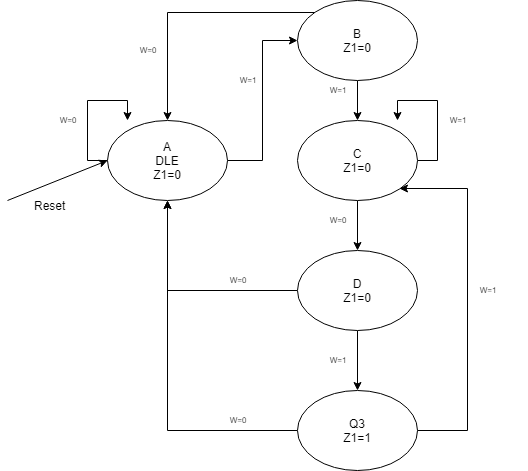
\includegraphics[scale=0.5]{../Exercise2/EJ2MOORE}
\caption{\color{cyan}Moore's State Machine, for detecting the sequence 1-1-0-1.}
\label{MOOREFSM}
\end{figure}

From above's diagram (the one in figure \ref {MOOREFSM}), the following table \ref {measej1} is obtained. 
\begin{table}[H]
\begin{center}
\begin{tabular}{|c|c c c|c|}
\hline
Present State & & Next State & & Output z \\
 & w=0 & & w=1 &   \\
\hline
\hline
A & A & & B & 0   \\
\hline
B & A & & C & 0   \\
\hline
C & D & & C & 0   \\
\hline
D & A & & E & 0   \\
\hline
E & A & & C & 1   \\
\hline
\hline
\end{tabular}
\end{center}
\caption{\label{measej1}\color{cyan}Moore's Next States and Outputs.}
\end{table}

The present state is represented as a 3 bit vector y: (y3,y2,y1) while the next state is represented as Y: (Y3,Y2,Y1). From the previous table \ref {measej1} the following Karnaugh maps are used to get to simple logic expressions. The first Karnaugh map is to get Y1, the second one for Y2, the third one for Y3 and the last one for the output z.

\begin{center} 
        \begin{Karnaugh}
            %cada 4 es una fila, la col 3 es la 4ta columna y 3fila es la 4 fila
            \contingut{
            0,0,1,0,
            0,X,X,X,
            1,0,0,0,
            0,X,X,X}
            \implicant{2}{6}{red}
            \implicant{8}{8}{green}
%            \implicant{12}{8}{orange}
%            \implicantdaltbaix[3pt]{1}{9}{blue}
            %\implicantcantons[2pt]{orange}
            %\implicantcostats{4}{14}{green}
        \end{Karnaugh}
    \end{center}



\begin{center}
        \begin{Karnaugh}
            %cada 4 es una fila, la col 3 es la 4ta columna y 3fila es la 4 fila
            \contingut{
            0,0,1,0,
            0,X,X,X,
            0,1,1,0,
            1,X,X,X}
            \implicant{2}{10}{red}
            \implicant{12}{14}{green}
%            \implicant{12}{8}{orange}
            \implicant{13}{9}{blue}
%            \implicantdaltbaix[3pt]{1}{9}{blue}
            %\implicantcantons[2pt]{orange}
            %\implicantcostats{4}{14}{green}
        \end{Karnaugh}
    \end{center}
  
  
\begin{center}
        \begin{Karnaugh}
            %cada 4 es una fila, la col 3 es la 4ta columna y 3fila es la 4 fila
            \contingut{
            0,0,0,0,
            0,X,X,X,
            0,0,0,1,
            0,X,X,X}
            \implicant{15}{11}{red}
%            \implicant{12}{14}{green}
%%            \implicant{12}{8}{orange}
%            \implicant{13}{9}{blue}
%            \implicantdaltbaix[3pt]{1}{9}{blue}
            %\implicantcantons[2pt]{orange}
            %\implicantcostats{4}{14}{green}
        \end{Karnaugh}
    \end{center}
    
   
    \begin{center}
        \begin{Karnaughvuit}
            %cada 4 es una fila, la col 3 es la 4ta columna y 3fila es la 4 fila
            \minterms{4}
        \maxterms{0,1,2,3}
        \indeterminats{5,6,7}
            \implicant{4}{6}{red}
%            \implicant{12}{14}{green}
%%            \implicant{12}{8}{orange}
%            \implicant{13}{9}{blue}
%            \implicantdaltbaix[3pt]{1}{9}{blue}
            %\implicantcantons[2pt]{orange}
            %\implicantcostats{4}{14}{green}
        \end{Karnaughvuit}
    \end{center}

From the Karnaugh maps, we get to the following expressions:
$$Y1 = \overline{y1} (\overline{y2}   \overline{y3}  w + y2 \overline{w})$$
$$Y2 = y2  \overline{y1} + w (y3 + \overline{y2}  y1)$$
$$y3 = y1  y2  w $$
$$z = y3 $$


\subsection{\color{purple}Mealy Type State Machine}

In figure \ref {MealyEFSM} it is represented the sequence detection with the Mealy's state machine.

\begin{figure}[H]
\centering
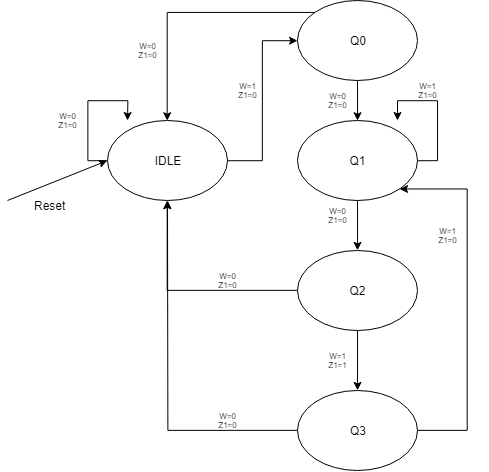
\includegraphics[scale=0.5]{../Exercise2/EJ2MEALY}
\caption{\color{cyan}Mealy's State Machine, for detecting the sequence 1-1-0-1.}
\label{MealyEFSM}
\end{figure}

It can be seen how in this case, the transition between one state to another now also causes a change in the output. It doesn't wait to get to the new state in order to change it. The following table is obtained from above's diagram in figure \ref {measej2} .
\begin{table}[H]
\begin{center}
\begin{tabular}{|c|c c c|c c c|}
\hline
Present State & & Next State & & & Output z & \\
 &  & & & & depending on w&  \\
 & w=0 & & w=1 & w=0& &w=1  \\
\hline
\hline
A & A & & B & 0 & & 0   \\
\hline
B & A & & C & 0 & & 0   \\
\hline
C & D & & C & 0 & & 0 \\
\hline
D & A & & E & 0 & & 1  \\
\hline
E & A & & C & 0 & & 0 \\
\hline
\hline
\end{tabular}
\end{center}
\caption{\label{measej2}\color{cyan}Mealy's Next States and Outputs.}
\end{table}
